\documentclass{article}
\usepackage[utf8]{inputenc}
\usepackage{graphicx}

\title{Tugas Database 2}
\author{Dinda Anik Masruro}
\date{1 November 2019}

\begin{document}

\maketitle

\section{Langkah-langkah Membuat Aplikasi Pada Oracle Apex Dengan Data Mahasiswa}
\item 1. Login
\begin{center}
    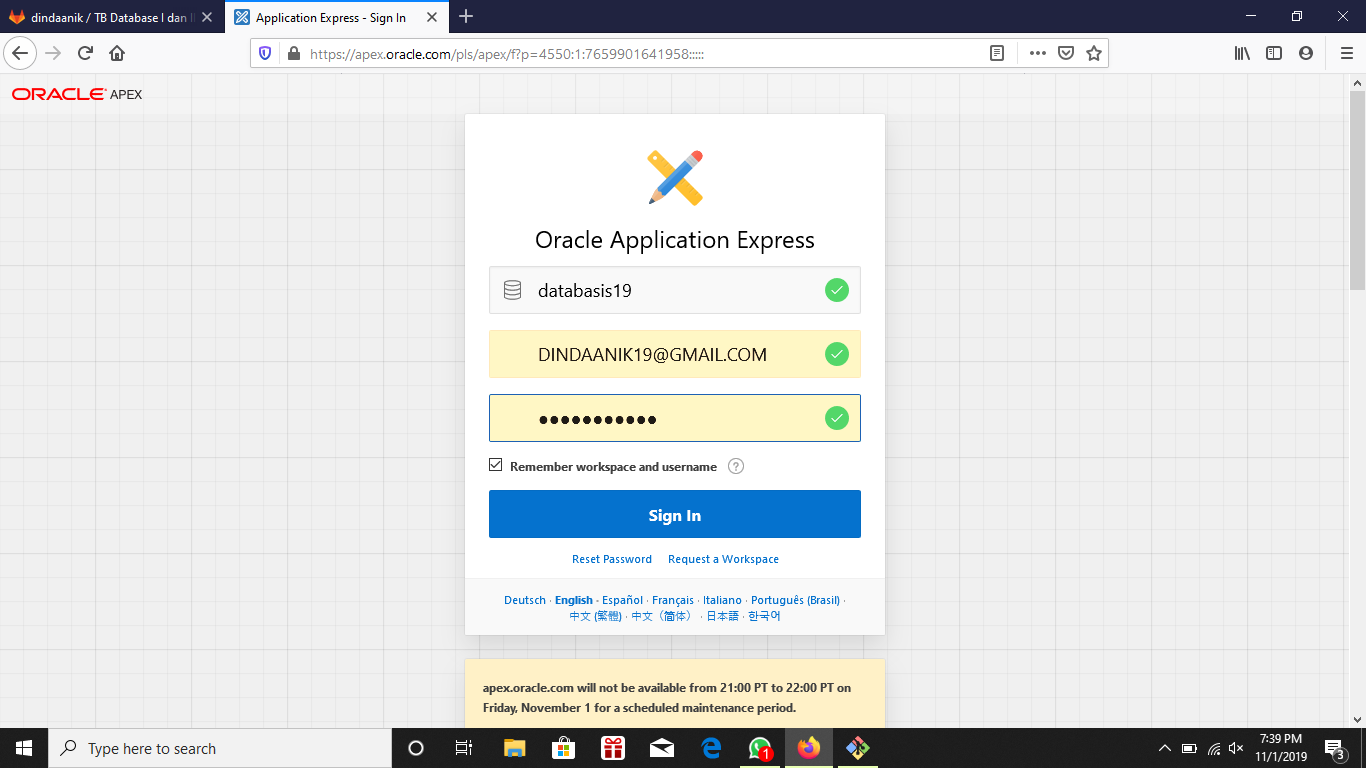
\includegraphics[width=10cm\textwidth]{gambar/1.png}
\end{center}
\item 2. Pilih app builder
\begin{center}
 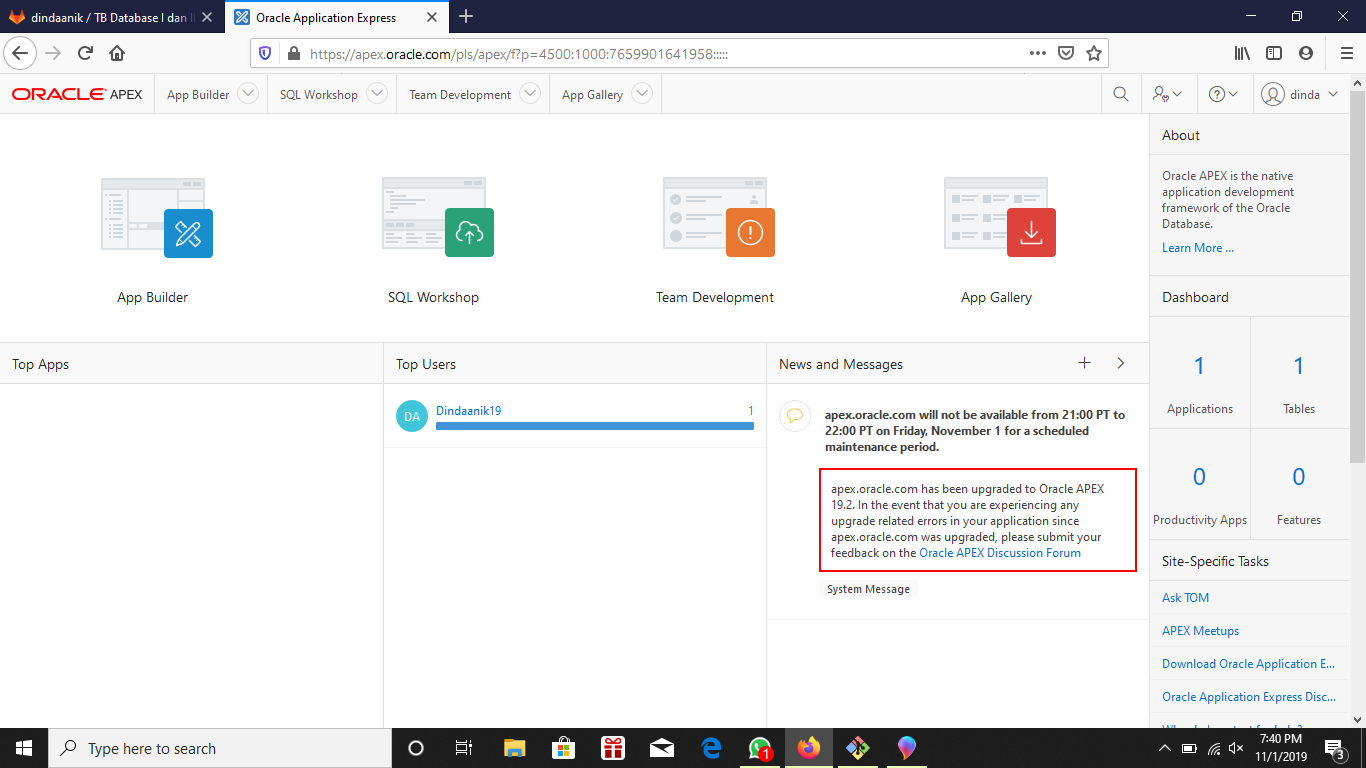
\includegraphics[width=10cm\textwidth]{gambar/2b.png}
\end{center}
\item 3. Untuk memasukkan data dari pc, kita pilih create.
\begin{center}
    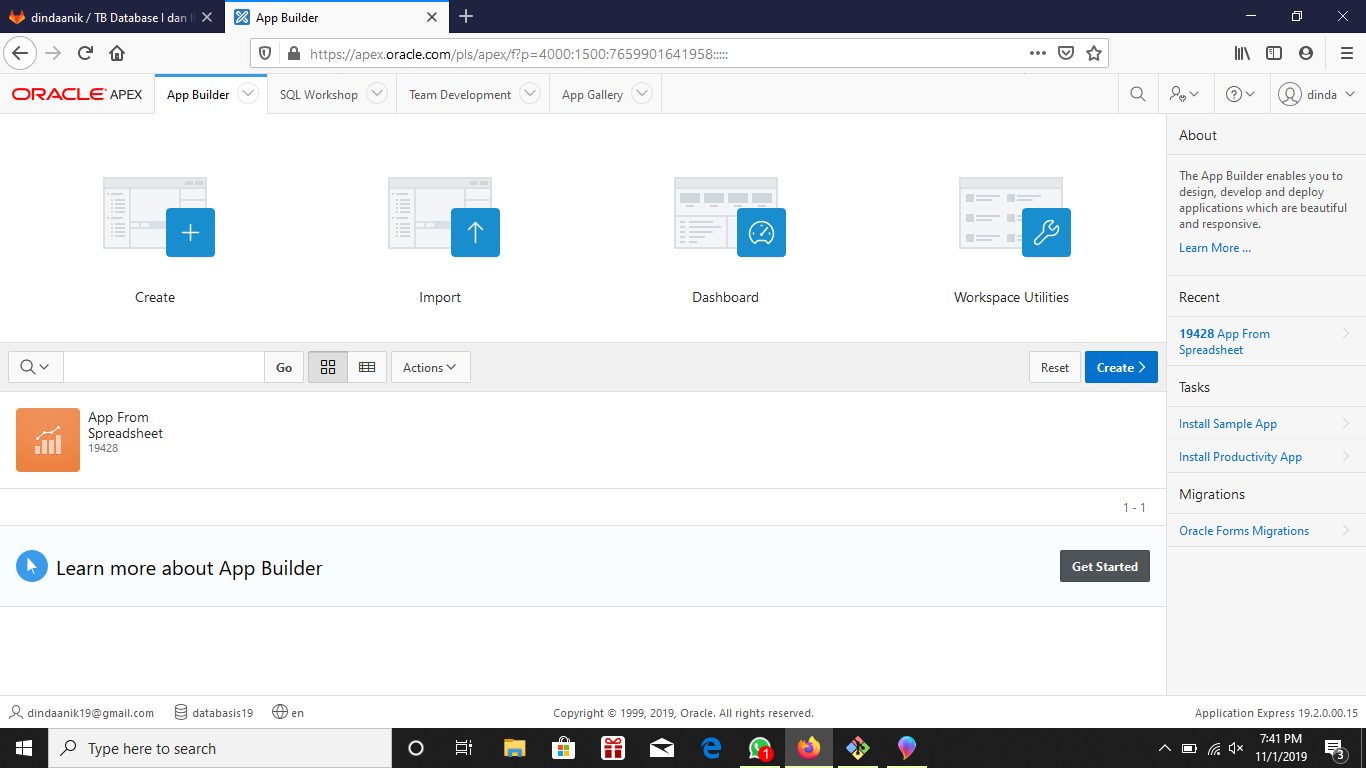
\includegraphics[width=10cm\textwidth]{gambar/3.png}
 \end{center}
 \item 4. Untuk memasukkan data kita pilih From a le ,jika sudah kita pilih data
mahasiswa yang ingin dimasukkan.
\begin{center}
 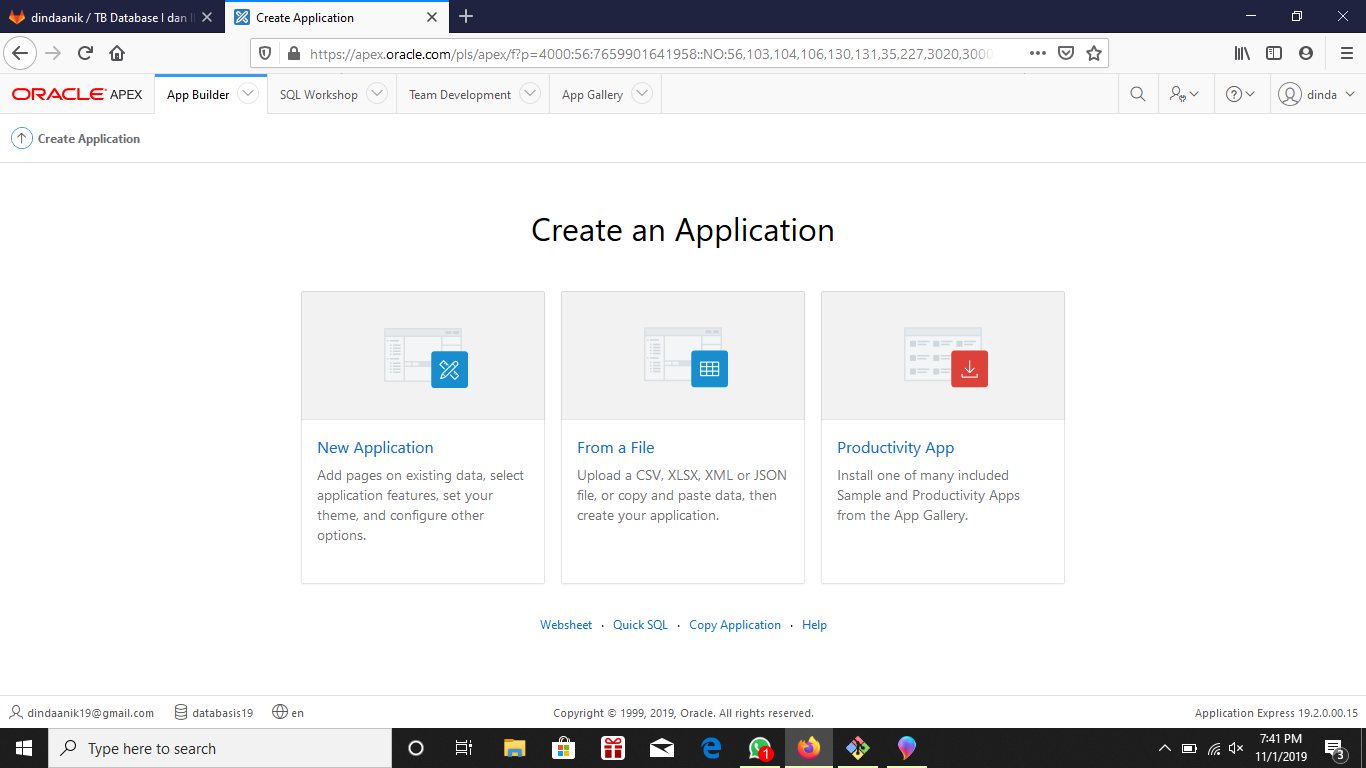
\includegraphics[width=10cm\textwidth]{gambar/4.png}
\end{center}
 \item 5. Jika data telah berhasil di input maka akan muncul tampilan
\begin{center}
 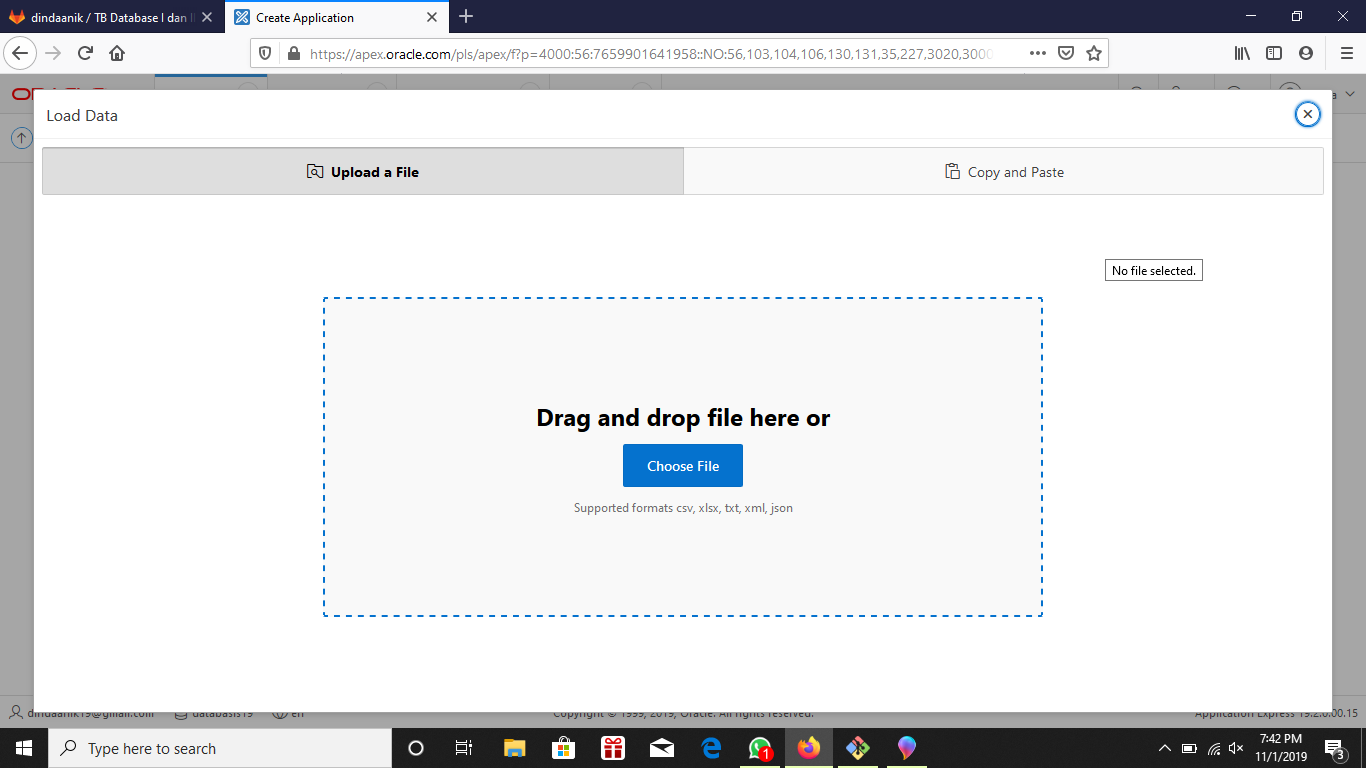
\includegraphics[width=10cm\textwidth]{gambar/5.png}
 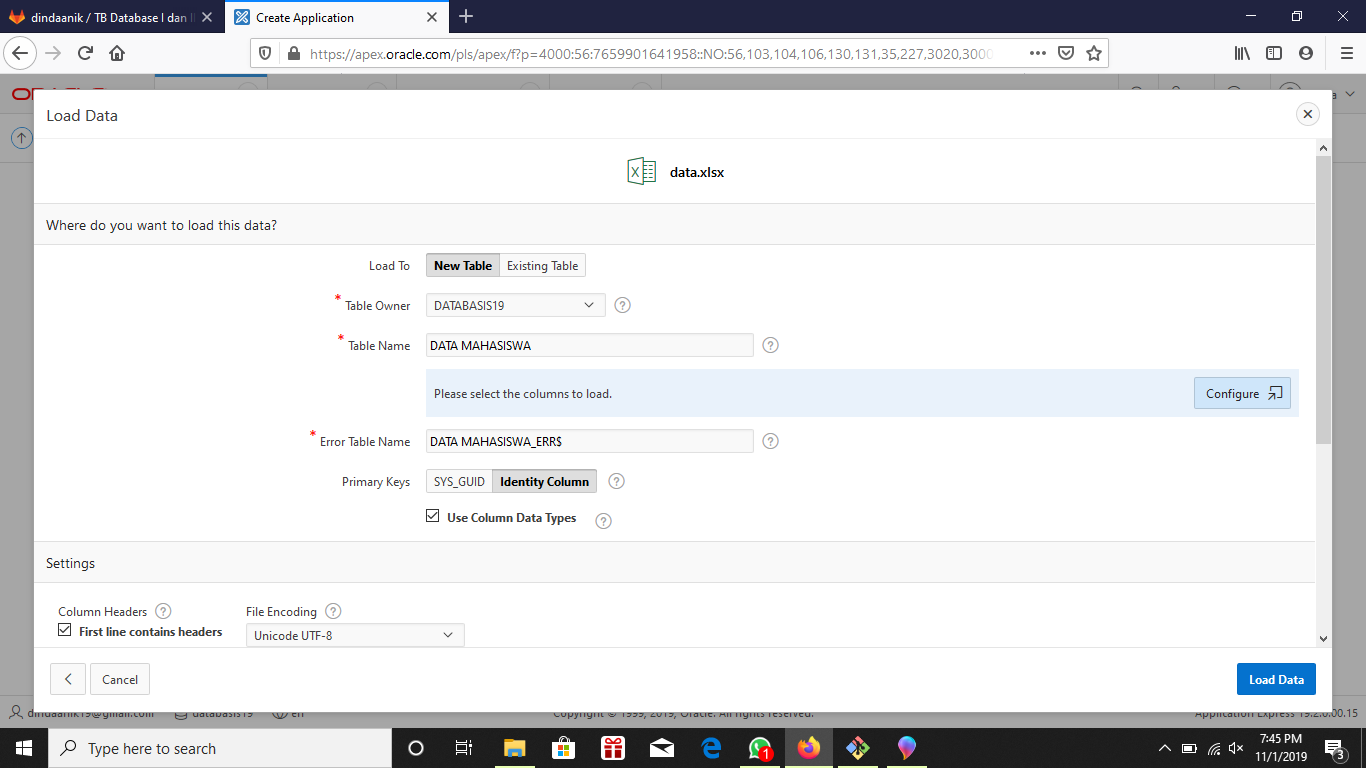
\includegraphics[width=10cm\textwidth]{gambar/6.png}
\end{center}
\item 6. Kita pilih save changes..untuk menyipan data yang telah diinput.
\begin{center}
 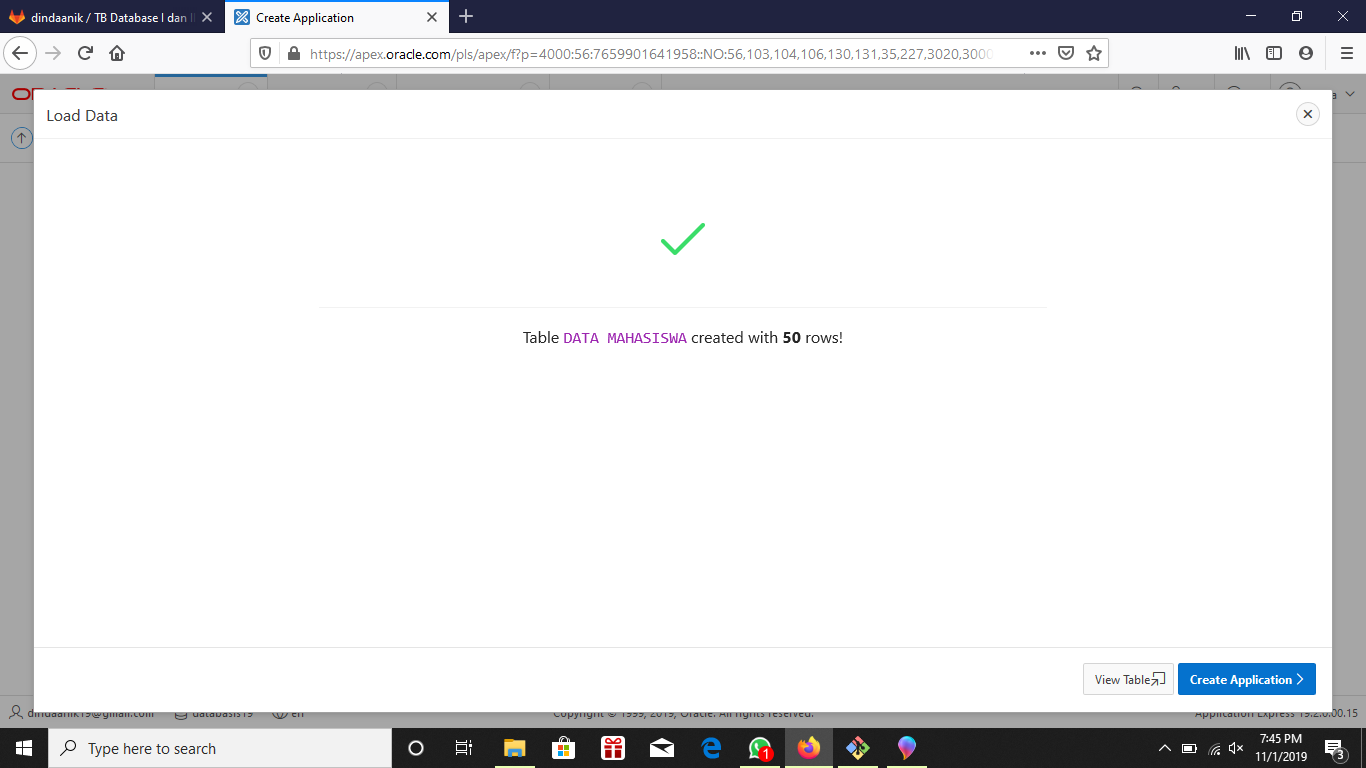
\includegraphics[width=10cm\textwidth]{gambar/7.png}
\end{center}
\newpage
\item 7. Selanjutnya kita pilih create apllication,jika sudah tampil seperti ini 
\begin{center}
 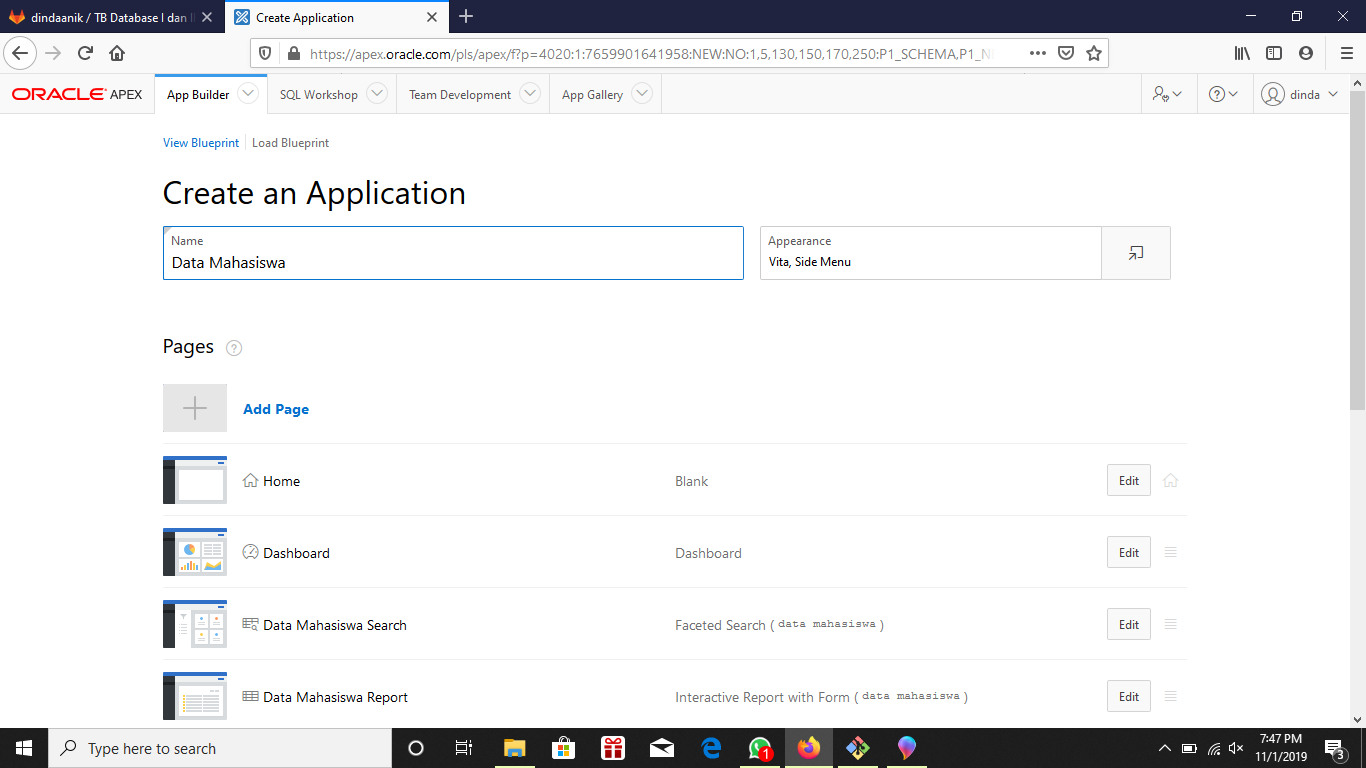
\includegraphics[width=10cm\textwidth]{gambar/8.png}
\end{center}
\item 8. etelah itu kita kembali ke menu utama dan dan memilih check list all.
\begin{center}
 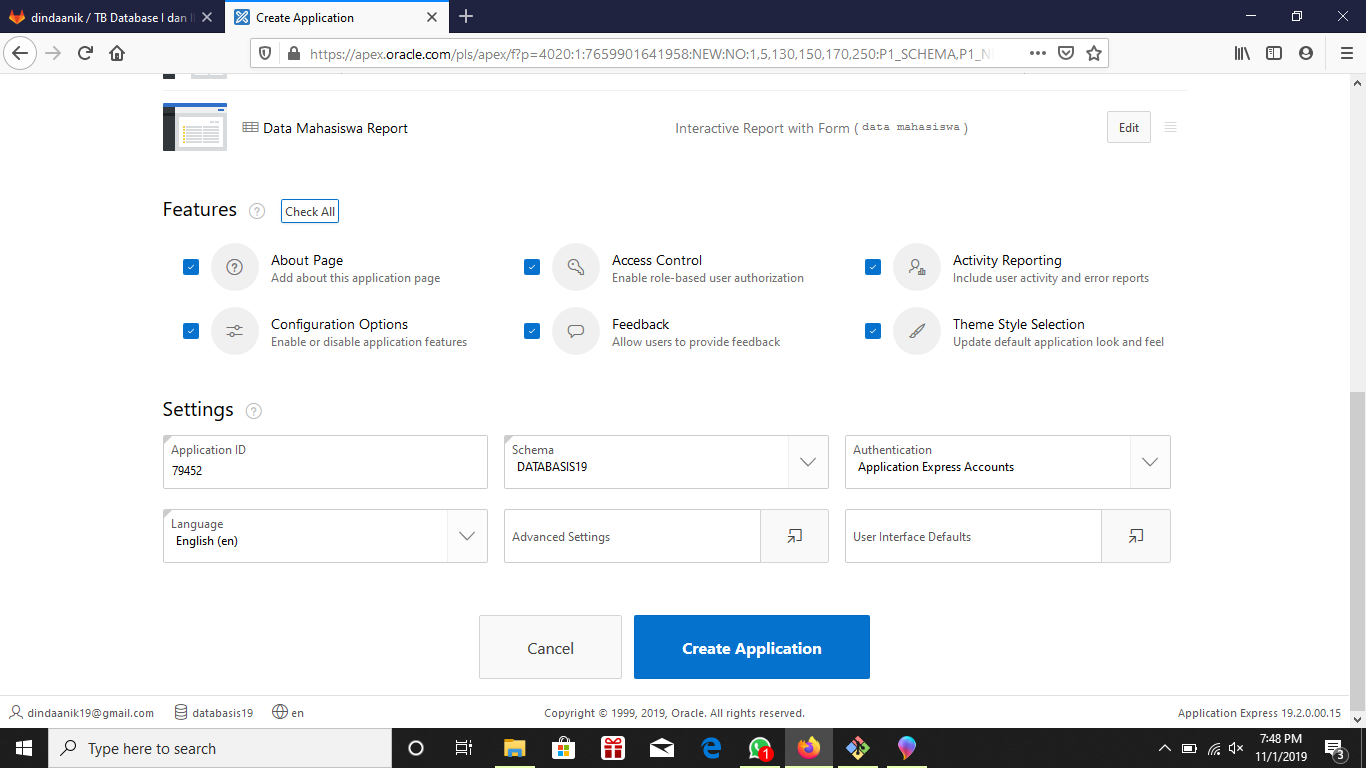
\includegraphics[width=10cm\textwidth]{gambar/9.png}
\end{center}
\item 9. maka akan tampul menu seperti dibawah ini
\begin{center}
 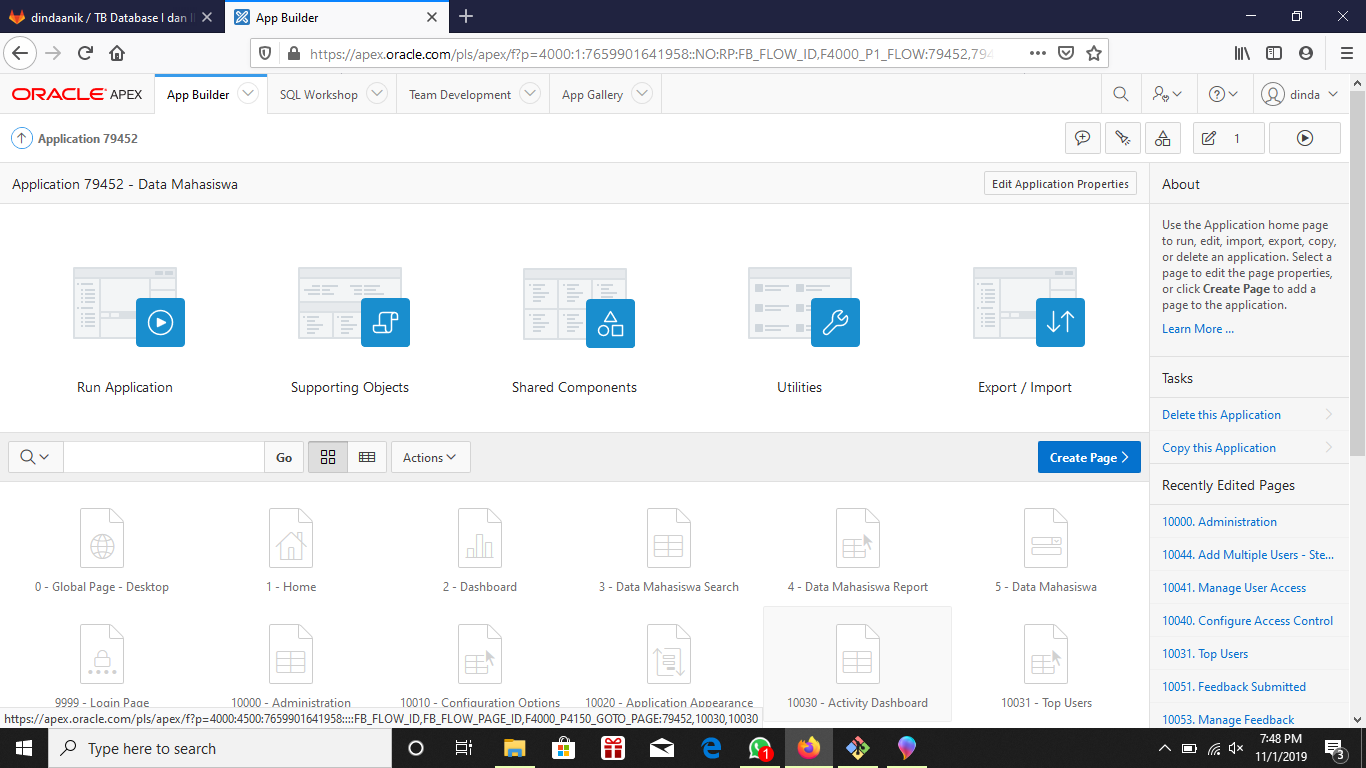
\includegraphics[width=10cm\textwidth]{gambar/10.png}
\end{center}
\item 10.Setelah kita run application maka akan muncul form login.kita isi email
dan password oracle apex. 
\begin{center}
 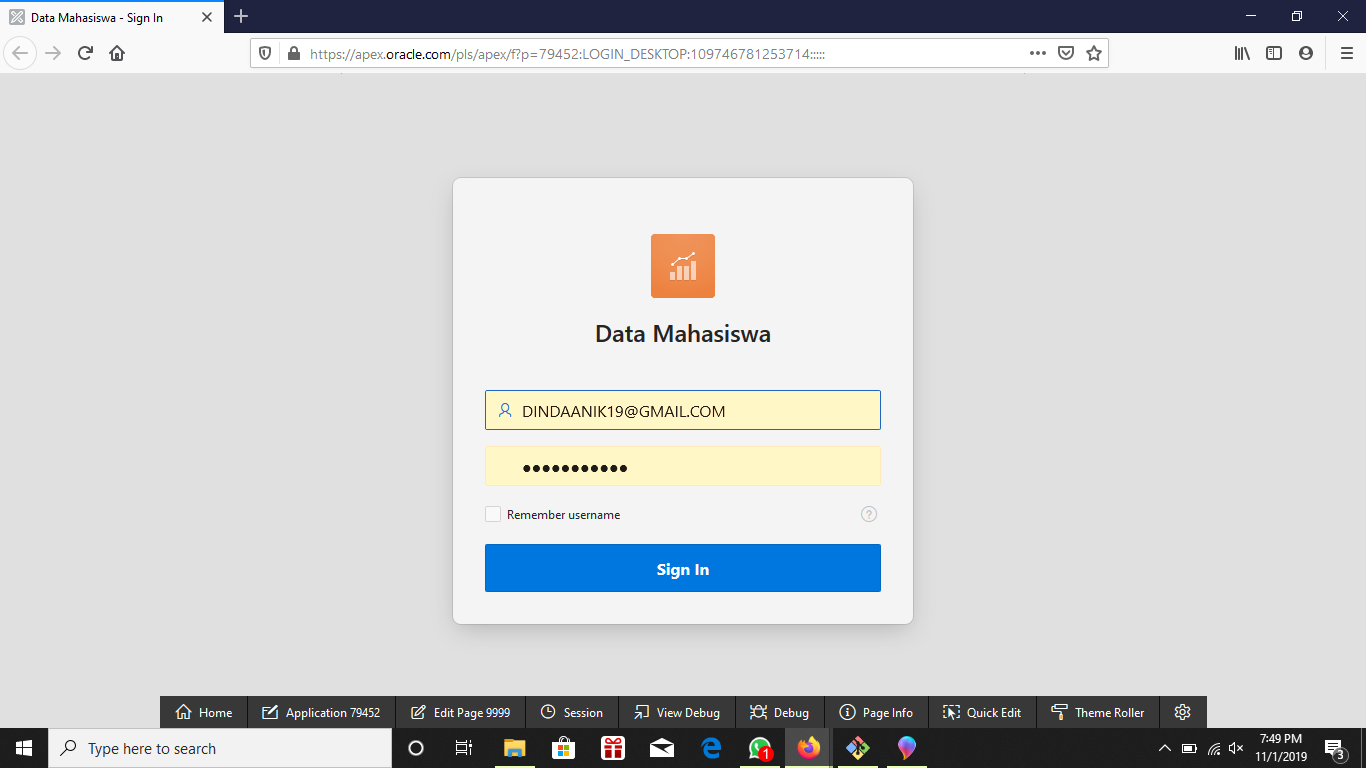
\includegraphics[width=10cm\textwidth]{gambar/11.png}
\end{center}
\item 11.jika telah berhasil masuk
\begin{center}
 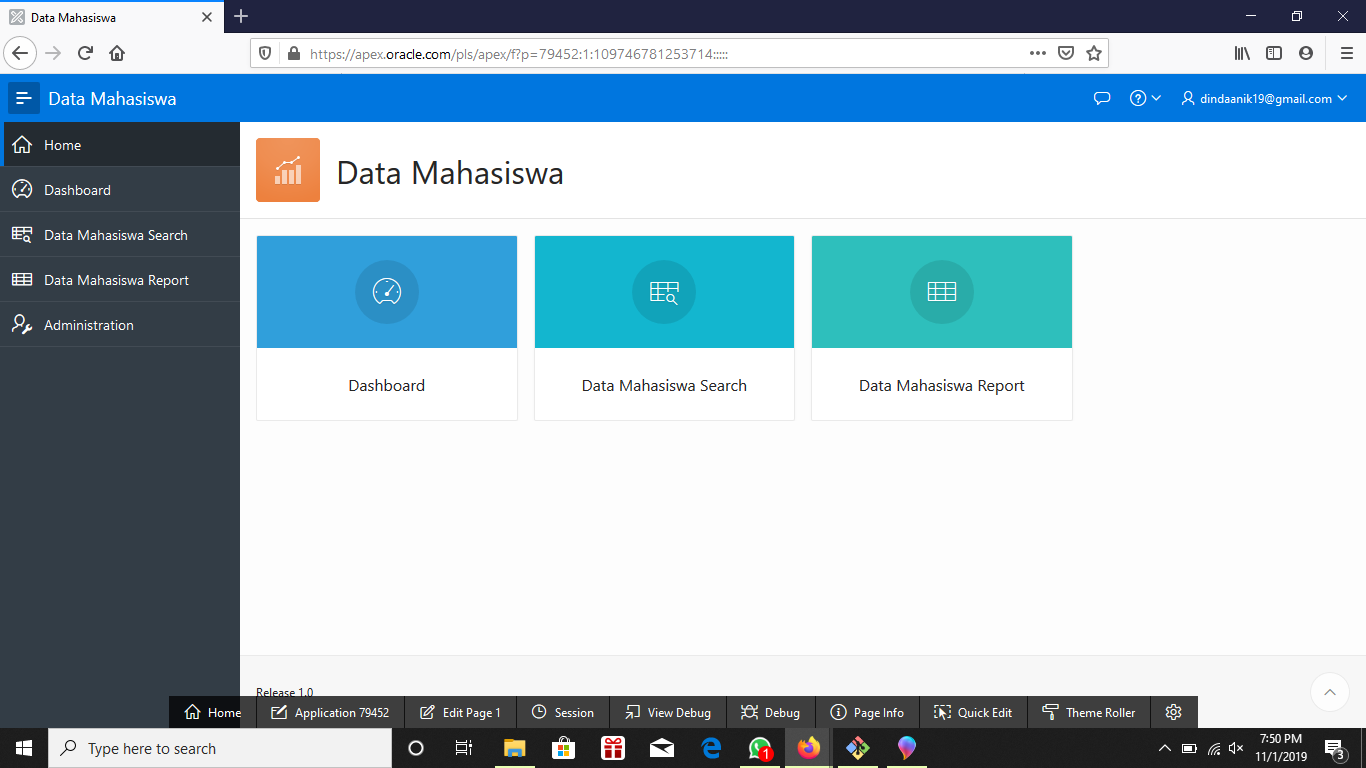
\includegraphics[width=10cm\textwidth]{gambar/12.png}
\end{center}
\item workspace: databasis19
\item password: dinda181205 
\end{document}
